\documentclass{beamer}
\usepackage{fancyvrb}
\usepackage{hyperref}
\usepackage{tikz}
\usepackage{tikz-qtree}

\usepackage{graphicx}


\newcommand{\bi}{\begin{itemize}}
\newcommand{\li}{\item}
\newcommand{\ei}{\end{itemize}}

\newcommand{\sect}[1]{
\section{#1}
\begin{frame}[fragile]\frametitle{#1}
}

\mode<presentation>
{
%  \usetheme{Madrid}
  % or ...

%  \setbeamercovered{transparent}
  % or whatever (possibly just delete it)
}

\usepackage[english]{babel}

\usepackage[latin1]{inputenc}

\title[RPN Calculator]
{
RPN Calculator
}

\subtitle{} % (optional)

\author[Geoffrey Matthews]
{Geoffrey Matthews}
% - Use the \inst{?} command only if the authors have different
%   affiliation.

\institute[WWU/CS]
{
  Department of Computer Science\\
  Western Washington University
}
% - Use the \inst command only if there are several affiliations.
% - Keep it simple, no one is interested in your street address.

\date{\today}

% If you have a file called "university-logo-filename.xxx", where xxx
% is a graphic format that can be processed by latex or pdflatex,
% resp., then you can add a logo as follows:

%\pgfdeclareimage[height=0.5cm]{university-logo}{WWULogoProColor}
%\logo{\pgfuseimage{university-logo}}

% If you wish to uncover everything in a step-wise fashion, uncomment
% the following command: 

%\beamerdefaultoverlayspecification{<+->}

\begin{document}

\begin{frame}
  \titlepage
\end{frame}

\sect{Expressing arithmetic trees}

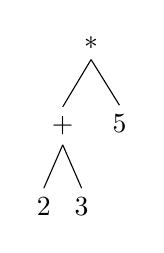
\begin{tikzpicture}
  \Tree [.$*$
    [.$+$
      [.2 ]
      [.3 ]
    ]
    [.5 ]
  ]  
\end{tikzpicture}
\hfill
\begin{minipage}[b]{2.5in}\footnotesize
\begin{verbatim}
  ((2 + 3) * 5)

  2 + 3 * 5            <= Infix

  * + 2 3 5            <= Prefix

  2 3 + 5 *            <= Postfix
\end{verbatim}
\end{minipage}

\vfill

\hrulefill

\vfill

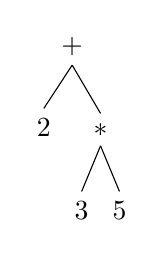
\begin{tikzpicture}
  \Tree [.$+$
    [.2 ]
    [.$*$
      [.3 ]
      [.5 ]
    ]
  ]  
\end{tikzpicture}
\hfill
\begin{minipage}[b]{2.5in}\footnotesize
\begin{verbatim}
  (2 + (3 * 5))

  2 + 3 * 5            <= Infix

  + 2 * 3 5            <= Prefix

  2 3 5 * +            <= Postfix
\end{verbatim}
\end{minipage}
\end{frame}


\sect{Expressing arithmetic trees}
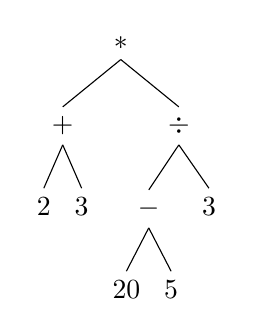
\begin{tikzpicture}
  \Tree [.$*$
    [.$+$
      [.2 ]
      [.3 ]
    ]
    [.$\div$
      [.$-$
        [.20 ]
        [.5 ]
      ]
      [.3 ]
    ]
  ]  
\end{tikzpicture}\hfill
\begin{minipage}[b]{2.5in}\footnotesize
\begin{verbatim}
  ((2 + 3) * ((20 - 5) / 3))

  2 + 3 * 20 - 5 / 3

  * + 2 3 / - 20 5 3

  2 3 + 20 5 - 3 / *
\end{verbatim}
\end{minipage}

\end{frame}

\sect{Parsing postfix arithmetic expressions}
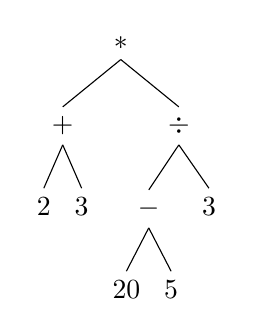
\begin{tikzpicture}
  \Tree [.$*$
    [.$+$
      [.2 ]
      [.3 ]
    ]
    [.$\div$
      [.$-$
        [.20 ]
        [.5 ]
      ]
      [.3 ]
    ]
  ]  
\end{tikzpicture}\hfill
\begin{minipage}{2.5in}
\[
\underbrace{
  \overbrace{2\ 3\ +}^{e_1}
  \underbrace{\overbrace{\ 20\ 5\ -}^{e_2}\ 3\ /}_{e_3}\ *
  }_{e_4}
\]
\vspace{1cm}


\end{minipage}

\vfill

\bi
\li Postfix grammar is LL(1):
\begin{align*}
  D &\rightarrow 0 \mid 1 \mid 2 \mid 3 \mid ... \\
  N &\rightarrow DN \mid D \\
  O &\rightarrow + \mid - \mid * \mid / \\
  E &\rightarrow N \mid E\ E\ O
\end{align*}
\ei

\end{frame}


\sect{Evaluating arithmetic trees}
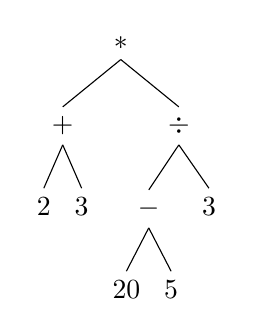
\begin{tikzpicture}
  \Tree [.$*$
    [.$+$
      [.2 ]
      [.3 ]
    ]
    [.$\div$
      [.$-$
        [.20 ]
        [.5 ]
      ]
      [.3 ]
    ]
  ]  
\end{tikzpicture}\hfill
\begin{minipage}{2.5in}
\begin{verbatim}
  2 3 + 20 5 - 3 / *
\end{verbatim}
\end{minipage}

\vfill

\bi
\li Postfix makes it easy to build an interpreter.
\li We assume we have a stack for numbers.
\li If it's a number, push onto a stack.
\li If it's an operator:
\bi
\li Pop the top two elements of the stack
\li Apply the operator to the two numbers
\li Push the result onto the stack
\ei
\li The answer will be on top of the stack.
\ei

\end{frame}

\sect{Evaluating arithmetic trees}
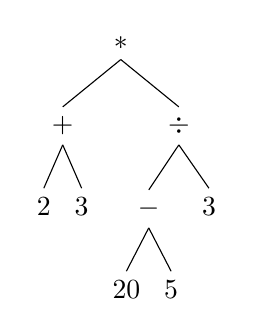
\begin{tikzpicture}
  \Tree [.$*$
    [.$+$
      [.2 ]
      [.3 ]
    ]
    [.$\div$
      [.$-$
        [.20 ]
        [.5 ]
      ]
      [.3 ]
    ]
  ]  
\end{tikzpicture}\hfill
\begin{minipage}{2.5in}
\begin{verbatim}
  2 3 + 20 5 - 3 / *
\end{verbatim}
\end{minipage}

\vfill

\bi
\li Note that we can also evaluate numbers while parsing:
\bi
\li Initialize an accumulator variable with 0.
\li For each digit:
\bi
\li Multiply the accumulator by 10
\li Add the digit
\ei
\ei

\[
6253 =
(((6 \times 10) + 2) \times 10) + 5) \times 10) + 3
\]
\pause

\li We ignore real numbers, negative numbers, {\em etc.}
\ei
\end{frame}

\end{document}
